\documentclass[aspectratio=169]{beamer}
\usepackage{standalone}
\usepackage{amsmath}
\usepackage{bm}

\usepackage{stmaryrd}
\usepackage{listings}
\usepackage{bussproofs}
\usepackage[T2A,T1]{fontenc}
\newcommand\cyr{\fontencoding{T2A}\selectfont} % \fontfamily{Tempora-TLF}}


\usepackage[hyperref=auto,style=alphabetic,backend=bibtex]{biblatex}
\addbibresource{kwarcpubs.bib}
\addbibresource{extpubs.bib}
\addbibresource{extcrossrefs.bib}
\addbibresource{bib.bib}
\usepackage{appendixnumberbeamer}
\usepackage{tikz}
\usepackage{tikz-qtree}
\usetikzlibrary{shapes.geometric} 
\usetikzlibrary{positioning}
\usetikzlibrary{arrows}
\usetikzlibrary{arrows.meta}

\usetheme{Pittsburgh}
% \setbeamertemplate{footline}[frame number]
\setbeamertemplate{footline}{\hfill\insertframenumber\,/\,\inserttotalframenumber\quad\strut}
\setbeamertemplate{navigation symbols}{}
\usecolortheme{beaver}
\setbeamertemplate{frametitle}[default][left]
% \setbeamersize{text margin left=3em}

\usepackage{utils/colors}
\usepackage[forbeamer]{utils/basic}
\usepackage{utils/operators}
\usepackage{utils/mylstmisc}
\usepackage{utils/lstmmt}

% \lstset{basicstyle=\ttfamily}
% \lstset{commentstyle=\itshape\color{commentfont}}
% \definecolor{codegray}{rgb}{0.9,0.9,0.9}
\lstset{basicstyle=\sf,columns=fullflexible}
\lstset{numberstyle=\tiny}
\lstset{language={[LaTeX]TeX}}
\lstset{literate=--1}

\title{Helping Humans Align Efficiently}

\author{{\bf Jan Frederik Schaefer}, Michael Kohlhase}
\institute{FAU Erlangen-N\"urnberg}
\date{Workshop on Math Datasets: alignments and comparisons (ALIGN2025)\\Brasilia, Brazil\\October 10, 2025}

\def\texthl#1{\colorbox{yellow!50!red!70}{#1}}

\begin{document}

\frame\titlepage



\begin{frame}[fragile]
    \frametitle{Introduction}
    \renewcommand\arraystretch{1.2}%\setlength\minrowclearance{2.4pt}
    \begin{itemize}
        \item Alignments make math data FAIR \com{Findable, Accessible, Interoperable, Reusable}
        \item Example: % nat in text / wikidata / ontomathpro
            \begin{tabular}l
                \texttt{http://ontomathpro.org/omp2\#E2119} (``Natural number'')\\
                    \hline
                    \hline
                ``Let $n$ be a \texthl{natural number}.''\\
                    \hline
                    \hline
                    \pause
                \texttt{wd:Q21199} (``natural number'')\\
                \texttt{wd:Q28920044} (positive integers, i.e.\ natural numbers excluding 0)\\
                \texttt{wd:Q28920052} (non-negative integers, i.e.\ natural numbers including 0)\\
            \end{tabular}
            \pause
        \item Will need human aligners
        \item $\leadsto$ Idea: Tool supported workflow for efficient alignment
            \com{Inspired by ideas from Snify (Wednesday's talk)}
    \end{itemize}
\end{frame}

\begin{frame}
    \frametitle{Proposed Workflow}
    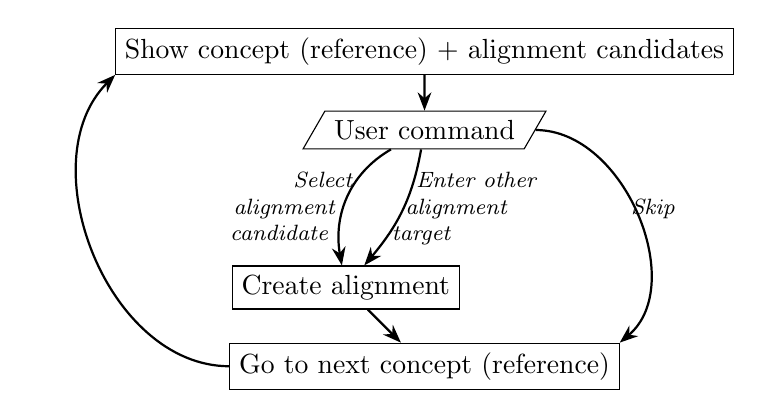
\begin{tikzpicture}
        \node[draw,rectangle] (show) at (0, 2) {Show concept (reference) + alignment candidates};
        \node[trapezium left angle=60, trapezium right angle=-60,trapezium,draw] (command) at (0, 1) {User command};
        \node[draw,rectangle] (create) at (-1, -1) {Create alignment};
        \draw[-Stealth,thick] (command) to[in=100,out=210] (create);
        \draw[-Stealth,thick] (command) to[in=50,out=260] (create);
        \node at (-1.65, 0) {\itshape\footnotesize\begin{tabular}rSelect\;\ \\alignment\quad\ \\candidate\quad\;\ \end{tabular}};
        \node at (0.5, 0) {\itshape\footnotesize\begin{tabular}l\quad Enter other\\\;\;alignment\\target\end{tabular}};
        \node[draw,rectangle] (next) at (0, -2) {Go to next concept (reference)};
        \draw[-Stealth,thick] (show) -- (command);
        \draw[-Stealth,thick] (create) -- (next);
        \draw[-Stealth,thick] (command) to[out=0,in=40] (next.north east);
        \node at (2.9, 0) {\itshape\footnotesize Skip};
        \draw[-Stealth,thick] (next) to[out=180,in=225] (show.south west);
    \end{tikzpicture}

    \pause
    \noindent\rule{\textwidth}{0.8pt}
    % {\centering ``Let $n$ be a \texthl{natural number}.''\par}
    \texttt{http://ontomathpro.org/omp2\#E2119} \\
    \begin{itemize}
        \item \texttt{[0] wd:Q21199}
        \item \texttt{[1] wd:Q28920044}
        \item \texttt{[2] wd:Q28920052}
    \end{itemize}
    \pause
    \noindent\rule{\textwidth}{0.8pt}
    \begin{itemize}
        \item How select candidates?
        \item More information needs to be displayed!
    \end{itemize}
    \textbf{$\bm\leadsto$ Solution: Concept Glossary}
\end{frame}


\begin{frame}[fragile]
    \frametitle{Concept Glossary}
    Have an entry for each concept with
    \begin{itemize}
        \item an identifier\com{for referencing/making the alignment}
        \item a (human-readable) description\com{so the user knows what the concept is}
        \item a set of verbalizations\com{for linking}
    \end{itemize}
    \pause
    \vspace{0.5em}\par
    \noindent\rule{\textwidth}{0.8pt}
    \vspace{0.5em}\par
    \textbf{For aligning}\\
    \quad\texttt{http://ontomathpro.org/omp2\#E2119}: 
    \texthl{``Natural number''} (en), ``{\cyr Натуральное число}'' (ru)\\
    \textbf{suggest e.g.}\\
    \quad\texttt{https://www.wikidata.org/wiki/Q28920044}\\
    \quad``\textit{positive integer} (integer greater than zero; natural number explicitly excluding zero)``\\
    \quad``positive integer'' (en), ``integer greater than zero'' (en), \texthl{``natural number''} (en), \textellipsis
\end{frame}

\begin{frame}
    \frametitle{Harvesters and Frontends}
    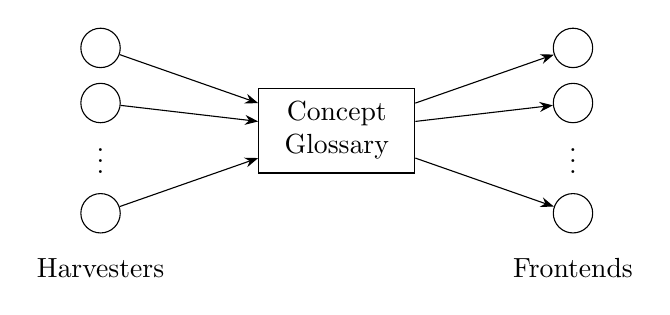
\begin{tikzpicture}[xscale=3, yscale=0.7]
        \node[circle,draw,minimum size=0.5cm] (h1) at (-1, 1.5) {};
        \node[circle,draw,minimum size=0.5cm] (h2) at (-1, 0.5) {};
        \node at (-1, -0.4) {$\vdots$};
        \node[circle,draw,minimum size=0.5cm] (h3) at (-1, -1.5) {};
        \node at (-1, -2.5) {Harvesters};
        \node[draw, rectangle] (catalog) at (0, 0) {\begin{tabular}cConcept\\Glossary\end{tabular}};
        \node[circle,draw,minimum size=0.5cm] (f1) at (1, 1.5) {};
        \node[circle,draw,minimum size=0.5cm] (f2) at (1, 0.5) {};
        \node at (1, -0.4) {$\vdots$};
        \node[circle,draw,minimum size=0.5cm] (f3) at (1, -1.5) {};
        \node at (1, -2.5) {Frontends};
        \draw[-Stealth] (h1) -- (catalog);
        \draw[-Stealth] (h2) -- (catalog);
        \draw[-Stealth] (h3) -- (catalog);
        \draw[-Stealth] (catalog) -- (f1);
        \draw[-Stealth] (catalog) -- (f2);
        \draw[-Stealth] (catalog) -- (f3);
    \end{tikzpicture}
    \vspace{2em}\par
    \begin{itemize}
        \item Different frontends depending on what we align
        \item Glossary as interface to harvesters
        \item $\leadsto$ harvesters and frontends can be implemented independently and combined freely\com{kind of}
    \end{itemize}
\end{frame}

\begin{frame}
    \frametitle{Prototype: Building on Snify}
    \begin{itemize}
        \item Snify: tool for efficient sTeX annotation\com{Presented on Wednesday}
        \item Today: building prototypes on Snify for WikiData alignment
    \end{itemize}
\end{frame}

\begin{frame}[fragile]
    \frametitle{A WikiData Harvester}
    {\centering Simple SPARQL query to get math concepts\com{18600 concepts}\vspace{2em}\par}
    \begin{lstlisting}[language=SPARQL]
SELECT DISTINCT ?item WHERE {
    { ?item wdt:P6104 wd:Q8487137 .
        FILTER NOT EXISTS {?item wdt:P31 wd:Q28920044. } .
        FILTER NOT EXISTS {?item wdt:P31 wd:Q5 }.
        FILTER NOT EXISTS {?item wdt:P31 wd:Q10376408 }.
    } UNION {VALUES ?item { wd:Q204 wd:Q199 wd:Q200 }}. 
  }
    \end{lstlisting}
\end{frame}

\begin{frame}
    \frametitle{Demo 1}
\end{frame}

\begin{frame}[fragile]
    \frametitle{Aligning Formulae}
    \textbf{WikiData has some notations $\to$ add them to glossary}
    \vspace{1em}\par
    \begin{itemize}
        \item identifier: \texttt{https://www.wikidata.org/wiki/Q167}
        \item description: ``constant ratio of the circumference of a circle to its diameter''
        \item verbalizations: \verb.\pi. (\LaTeX), $\pi$ (Unicode), ``pi'' (en), ``Archimedes' constant'' (en), \textellipsis
    \end{itemize}
    \vspace{1em}\par
    \pause
    \begin{itemize}
        \item Can annotate \LaTeX\ formulae
        \item Can annotate HTML documents (text/MathML formulae)
    \end{itemize}
\end{frame}

\begin{frame}
    \frametitle{Demo 2}
\end{frame}

\begin{frame}
    \frametitle{Sketch: Aligning OntoMathPro}
\end{frame}

\begin{frame}[fragile]
    \frametitle{Alignments Extend Glossary}
    \begin{itemize}
        \item Text/formula alignment yields new verbalization
        \item Transport verbalizations/notations across alignments
    \end{itemize}
    \vspace{1em}\par
    \textbf{Example:}\\
    \begin{enumerate}
        \item Align occurrence of \verb|\mathbb{N}| in a document with \texttt{wd:Q21199}
        \item Align \texttt{wd:Q21199} with \texttt{omp2:E2119}
        \item $\leadsto$ \verb|\mathbb{N}| is also a notation for \texttt{omp2:E2119}
    \end{enumerate}
\end{frame}

\begin{frame}
    \frametitle{Conclusion}
\end{frame}

\appendix
\begin{frame}[allowframebreaks,t]
    \frametitle{References}
    \printbibliography
\end{frame}



\end{document}
